\documentclass[aspectratio=1610]{beamer}
%\linespread{1.5}\selectfont

\usepackage{booktabs}
\usepackage{dcolumn}
\usepackage{float}
\usepackage{placeins}
\usepackage{lscape} 
\usepackage{tikz}
\usepackage[export]{adjustbox}
\usepackage{ragged2e}
\justifying
\usepackage{outlines}
\usepackage{amsmath}
\usepackage{booktabs}
\usepackage{float}
\usepackage{dcolumn}
\usepackage{longtable}
\usepackage{array}
\usepackage{multirow}
\usepackage{wrapfig}
\usepackage{float}
\usepackage{colortbl}
\usepackage{pdflscape}
\usepackage{tabu}
\usepackage{threeparttable}
\usepackage{caption}
%\captionsetup{font=footnotesize}
\usepackage{subcaption}
\usepackage{threeparttable}
\usepackage[normalem]{ulem}
\usepackage{makecell}
\usepackage{xcolor}
\usepackage{hyperref}
\hypersetup{
    colorlinks = true, 
    linkcolor = red, 
    urlcolor = teal, 
    citecolor = blue}

%\usepackage{caption}
%\captionsetup{labelformat=empty}
\usepackage{appendixnumberbeamer}
\renewcommand{\raggedright}{\leftskip=0pt \rightskip=20pt plus 0cm}
\setbeamercovered{transparent}

\DeclareUnicodeCharacter{0301}{\'{e}}
\DeclareUnicodeCharacter{2212}{-}
\DeclareUnicodeCharacter{0327}{\c}

\usepackage[backend = biber, style=authoryear, sorting = nty, maxcitenames=1]{biblatex}

\addbibresource{citations_sesmarias.bib}

\graphicspath{{~/OneDrive - University of Illinois - Urbana/Research/Projects/Sesmarias Brazil/Figures/Descriptive/}}

%\addbibresource[location = remote]{https://raw.githubusercontent.com/ViniOkadaSilva/Papers/master/Sesmarias/citations_sesmarias.bib}

\DeclareFieldFormat{citehyperref}{%
  \DeclareFieldAlias{bibhyperref}{noformat}% Avoid nested links
  \bibhyperref{#1}}

\DeclareFieldFormat{textcitehyperref}{%
  \DeclareFieldAlias{bibhyperref}{noformat}% Avoid nested links
  \bibhyperref{%
    #1%
    \ifbool{cbx:parens}
      {\bibcloseparen\global\boolfalse{cbx:parens}}
      {}}}

\savebibmacro{cite}
\savebibmacro{textcite}

\renewbibmacro*{cite}{%
  \printtext[citehyperref]{%
    \restorebibmacro{cite}%
    \usebibmacro{cite}}}

\renewbibmacro*{textcite}{%
  \ifboolexpr{
    ( not test {\iffieldundef{prenote}} and
      test {\ifnumequal{\value{citecount}}{1}} )
    or
    ( not test {\iffieldundef{postnote}} and
      test {\ifnumequal{\value{citecount}}{\value{citetotal}}} )
  }
    {\DeclareFieldAlias{textcitehyperref}{noformat}}
    {}%
  \printtext[textcitehyperref]{%
    \restorebibmacro{textcite}%
    \usebibmacro{textcite}}}

\renewcommand*{\nameyeardelim}{\addcomma\space}

\usepackage{setspace}
\usepackage{graphicx}

\newcommand{\tinytable}[1]{\textcolor{black}{\tiny \input{#1}}}

\graphicspath{{~/OneDrive - University of Illinois - Urbana/Research/Writing/git/Sesmarias/Pictures/}}

\beamertemplatenavigationsymbolsempty

%Information to be included in the title page:
\title{Portuguese Colonial Land Grants in Brazil: Long-term Effects on Inequality and Economic Development}
\author{Vinicius Okada da Silva}
\institute{AMRL}
\date{}

\setbeamertemplate{footline}[frame number]

\begin{document}


\begin{frame}[plain, noframenumbering]
	\titlepage
\end{frame}

\begin{frame}{Motivation}
    \begin{outline}
        \1 Inequality, in both land and income, is high in Brazil.
            \vspace{1mm}
            \2 ``\textcolor{red}{\textbf{Brazil has one of the highest levels of inequality of land distribution in the world}}. Inadequate access to land by the poor and insecure land tenure are factors behind rural poverty violence, human rights abuses, and exploitation of rural workers in conditions of servitude'' \parencite{Usaid2016-xs}
            \vspace{1mm}
            \pause 
            \2 ``\textcolor{red}{\textbf{An estimated 1\% of the population owns 45\% of all land in Brazil}}. Nearly five million families are landless.'' \parencite{Usaid2016-xs}
        \pause 
        \1 However, it is nothing new with land inequality already high in 1920 and 1960s agricultural censuses \parencites{Alston2010-cn}{Wigton-Jones2020-ex}.
    \end{outline}
\end{frame}

\begin{frame}{Research Question}
    \begin{outline}
        \1 How much of it can be traced to colonial institutions?
            \vspace{1mm}
            \2 Goal of this research would analyze the effects of colonial Portuguese land grants (\textit{sesmarias}) on long-term inequality in Brazil.
            \vspace{1mm}
            \2 Exploit \textbf{\textit{plausibly exogenous}} variation on where the \textit{sesmarias} could be granted during early colonization because of a treaty between Portugal and Spain (RDD). 
            \2 Exploit \textbf{variation of soil quality} for different types of production across colonial Brazil (IV).
            \vspace{1mm}
            \2 Still looking for more institutional details on other possible sources of exogenous variation that could help me get a better identification.
        \pause 
        \1 Early studies argued it led to the development of the ``\textcolor{red}{\textbf{economic aristocracy of the colonial society}}'' and the ``\textcolor{red}{\textbf{principal cause of [plantations]}}'' in Brazil \parencites[p.~36]{Lima2002-kd}[p.~48]{Da_Costa_Porto1979-dz}.
        \vspace{1mm}
        \1 ``Today the system of ownership and use of land is a \textcolor{red}{\textbf{continuation of the colonial system, with the \textit{sesmaria} becoming [plantations]}}" \parencite[p.~18]{Andrade1980-md}.
    \end{outline}
\end{frame}

\begin{frame}{History/Background}{Early Colonization}
    \begin{outline}
        \1 Land grants were given from 1530-1822, and often favored the Portuguese aristocracy \parencites[p.~16]{Diegues_Junior1959-ba}{Lobb1976-mc}
        \vspace{1mm}
        \pause 
        \1 Goal was to establish Portuguese presence in Brazil at a low cost for the Crown.
        \pause 
        \vspace{-2mm}
        \1 Technically, the only legal way to obtain lands in colonial Brazil.
            \2 Every land that was not donated as a \textit{sesmaria} was theoretically part of the public domain
            \2 Since the King owned the land, he could choose to distribute it to whomever he chose.
        \vspace{1mm}
        \pause 
        \1 Once the request was granted, it came with requirements such as developing the land.
        \vspace{1mm}
            \2 A good parallel to the U.S. would be the Homestead Act of 1862. 
    \end{outline}
\end{frame}

\begin{frame}{History/Background}{Request Process}
    \begin{outline}
        \1 Petitioner submits a letter for an unoccupied land detailing their qualifications (captain, governor, etc.)
        \vspace{1mm}
        \pause 
        \1 Governor reads it, and if accepted returns back a letter with the requirements for the petitioner to satisfy.
        \vspace{1mm}
        \pause 
        \1 Five years to develop the land
        \vspace{1mm}
        \pause 
        \1 If successful, upon an inspection, land was transferred to the \textit{sesmeiro}.
        \vspace{1mm}
        \pause 
        \1 Able to sell, pass down as inheritance, etc. 
        \pause 
        \1 \textbf{Currently, in the data, most of the requests were granted.} 
    \end{outline}
\end{frame}

\begin{frame}{Possible Channels}
    \begin{outline}
            \1 Land inequality $\Rightarrow$ only those with sufficient financial conditions were granted \textit{sesmarias}, and were often granted vast plots of land.
            \pause 
            \vspace{1mm}
            \1 Income inequality $\Rightarrow$ land was associated with wealth, fewer people with land lead to wealth accumulation by the few.
            \pause 
            \vspace{1mm}
            \1 Demographic Differences $\Rightarrow$ \textit{Sesmarias} often required African slaves, which could skew the demographics of a location.
            \pause 
            \vspace{1mm}
            % \2 Economic Development $\Rightarrow$ the lands granted were (supposed to be) developed by the owners, leading to the early economic development of an area.
            %\2 Urban development $\Rightarrow$ .
            \1 Political dominance $\Rightarrow$ Dominance by aristocrats often hampered efforts for local reform and investment.\footnote[frame,1]{``If the land was concentrated by a few owners, the \textit{latifundio} is created and it limits the number of settlers and the possibility of them entering the social class of \textit{senhores de engenho} or farmers \parencite[p.~40]{Bandecchi1963-uj}}
    \end{outline}
\end{frame}

\begin{frame}{Data}
    \label{data slide}
    \begin{outline}
        \1 Information of \textit{sesmarias} from the \href{http://plataformasilb.cchla.ufrn.br/}{Sesmarias of the Luso-Brazilian Empire Database} (Currently in progress) 
        \hyperlink{document example}{\beamerbutton{Doc. Example}}
        \hyperlink{data}{\beamerbutton{Data}}.
        \1 Brazilian Censuses (1872-2010)
            \vspace{1mm}
            \2 Possibility of exploring other demographic data from other sources (eg. \href{http://colonialpopulations.fcsh.unl.pt/mainEnglish.php}{Counting Colonial Populations})
            \vspace{1mm}
        \1 Brazilian Agricultural Censuses (First one in 1920).
        \vspace{2mm}
        \1 LandSat data to measure the current land usage (begins in 1985).
        \vspace{2mm}
        \1 Brazilian election results from 1889-1937 \href{https://projetohipol.wordpress.com/projetos/eleicoes-antes-da-democracia-dados-estatisticos-1889-1937/}{History of Political Institutions} (To be released).
        \vspace{2mm}
        \1 FAO GAEZ dataset for crop suitability.
    \end{outline}
\end{frame}

\begin{frame}{Treaty of Tordesillas (1494) and the Treaty of Madrid (1750)}
    \begin{figure}
        \centering
        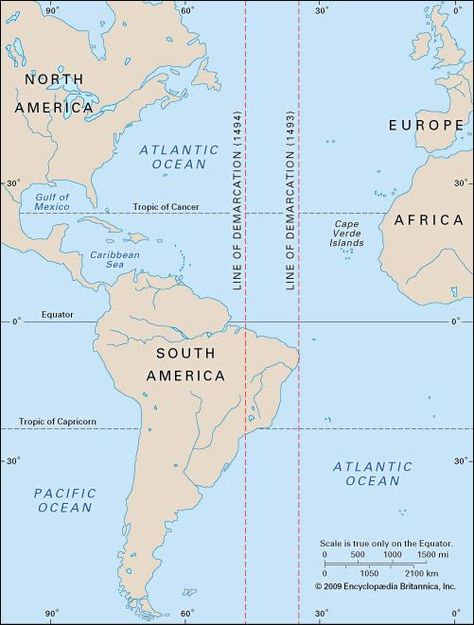
\includegraphics[width = .6\textheight]
        {treaty_tordesillas.jpeg}
        \centering
        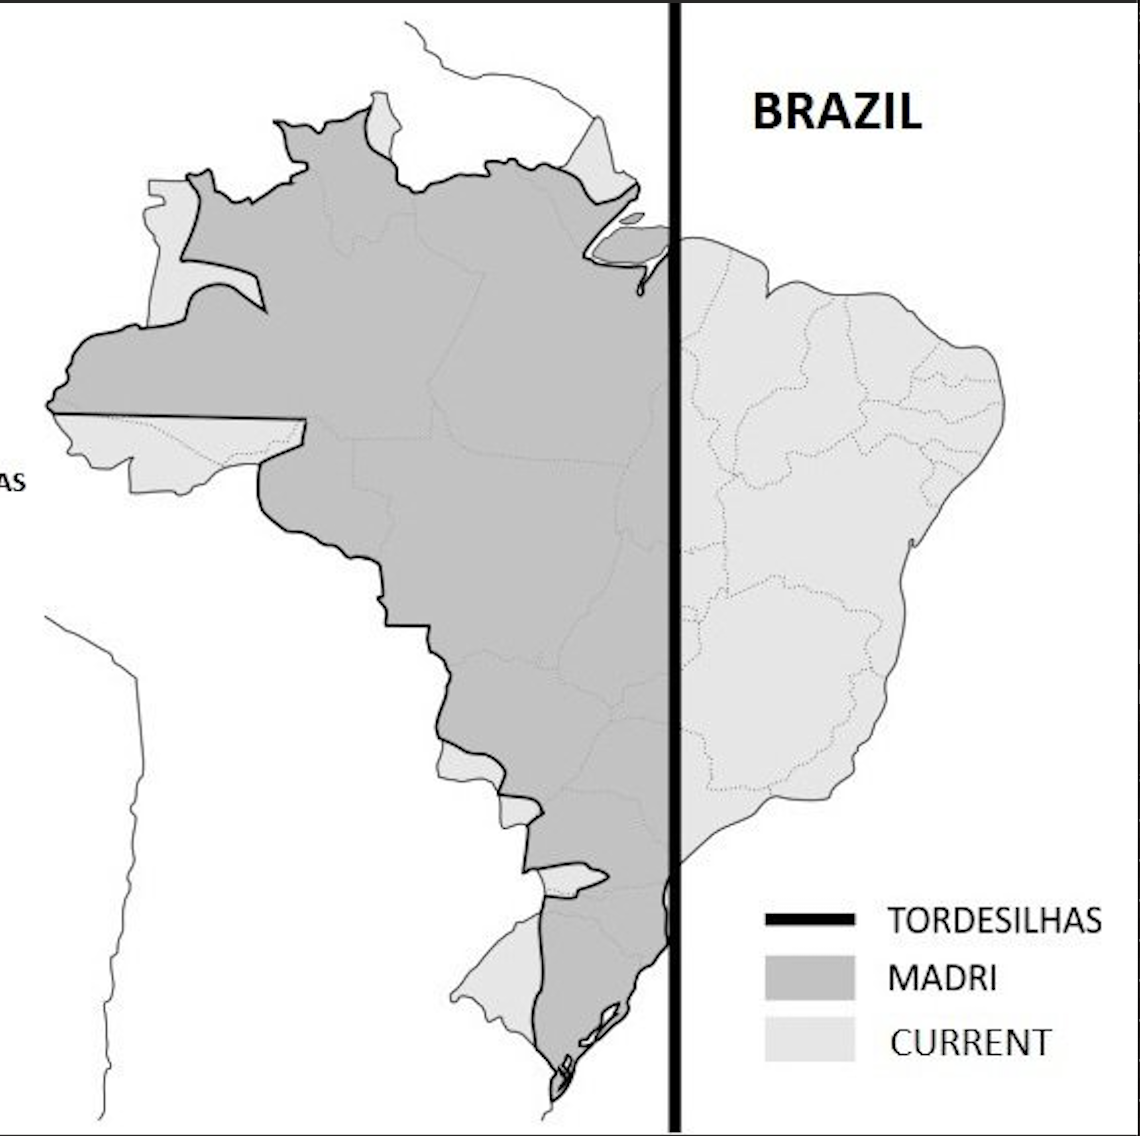
\includegraphics[width = .75\textheight]{treaty_madrid_v2.png}
    \end{figure}
\end{frame}

\begin{frame}{Identification Strategy I}{Fuzzy RDD Design}
    \begin{outline}
        \1 Estimate a Fuzzy RDD in which the probability a municipality has a \textit{sesmaria} is a function of whether it is located to the Portuguese side of the Treaty of Tordesillas (follows \cite{Laudares2022-vy} (WP)). 
    \end{outline}
    \vspace{3mm}
    First Stage:
    $$ Sesmarias_{m,s} = \delta \cdot TT_{m,s} + f(D_{m,s})+ \mu_s + X_{m,s} + \epsilon_{m,s} $$
    Second Stage:
    $$ Y_{m,s} = \beta \cdot \widehat{Sesmarias_{m,s}} + f(D_{m,s})+ \mu_s + X_{m,s} + \epsilon_{m,s}$$
\end{frame}

\begin{frame}{Identification Strategy II}{Instrumental Variable}
    \begin{outline}
        \1 Exploit exogenous land quality for certain types of requests, following \cite{Wigton-Jones2020-ex} (JEG).
        \1 Exclusion restriction requires that the suitability for a certain crop only affects outcomes in the future through the land grants.
    \end{outline}
    \vspace{3mm}
    First Stage:
    $$ Sesmarias_{m,s} = \delta \cdot Suitability_{m,s} + \mu_s + X_{m,s} + \epsilon_{m,s} $$
    Second Stage:
    $$ Y_{m,s} = \beta \cdot \widehat{Sesmarias_{m,s}} + \mu_s + X_{m,s} + \epsilon_{m,s}$$
\end{frame}

\begin{frame}{Yield Variation - Sugarcane}
    \centering
    \includegraphics[width=0.95\textwidth,height=0.95\textheight,keepaspectratio]
    {~/OneDrive - University of Illinois - Urbana/Research/Projects/Sesmarias Brazil/Figures/Descriptive/sugarcane_FAO_2010.png}
\end{frame}

%\begin{frame}{Identification Strategy}{Standard OLS}
%    \begin{outline}
%        \1 Most basic one would be standard OLS, repeated across various censuses.
%        $$ Y_{m,s} = \beta \cdot Sesmarias_{m,s} + X_{m,s} + \mu_s + \epsilon_{m,s}$$
%            \vspace{-5mm}
%            \2 $X_{m,s}$ would contain geographical characteristics and other pre-colonial measures. 
%            \2 $Sesmarias_{m,s}$ would be a measure of the fraction of land of a municipality that was granted through a \textit{sesmaria}.
%    \end{outline}
%\end{frame}

%\begin{frame}{Identification Strategy}{Standard OLS - Heterogeneity by Grant Request}
%    \begin{outline}
%        \1 Most basic one would be standard OLS, repeated across various censuses.
%        $$ Y_{m,s} = \beta_1 \cdot Sesmarias^{ag}_{m,s} + 
%        \beta_2 \cdot Sesmarias^{lv}_{m,s} + \beta_3 \cdot Sesmarias^{mn}_{m,s} + X_{m,s} + \mu_s + \epsilon_{m,s}$$
%            \vspace{-5mm}
%            \2 $X_{m,s}$ would contain geographical characteristics and other pre-colonial measures. 
%            \2 $Sesmarias^{type}_{m,s}$ would be a measure of the fraction of land of a municipality that was granted through a \textit{sesmaria} of a certain type (agricultural, livestock, and mining).
%    \end{outline}
%\end{frame}

\begin{frame}{Work to be Done}
    \label{work}
    \begin{outline}
        \1 Transcription of Manuscripts and information extraction are being done in Brazil.
            \vspace{1mm}
            \2 My state of \href{https://www.rosepepe.com.br/hotsite_acervo/sesmarias/}{Para} (\href{http://www.siaapm.cultura.mg.gov.br/modules/brtbusca/index.php?action=results&query=sesmarias&x=-722&y=-59}{and Minas Gerais}) has all the transcriptions $\Rightarrow$ only needed to extract the information.
            \vspace{0.5mm}
                \3 Machine Learning techniques to extract the information [Currently what I am working on]
                \vspace{0.5mm}
        \1 Georeferencing would be most of the work required.
            \vspace{1mm}
            \2 Look for a professional that works with Brazilian historical data.
        \1 Descriptive statistics from the current observations: 
        \\
        \hyperlink{contents}{\beamerbutton{Obs. State}}
        \hyperlink{year}{\beamerbutton{Year Dist.}}
        \hyperlink{size}{\beamerbutton{Size Dist.}}
    \end{outline}
\end{frame}

%\begin{frame}{Basic Descriptive Statistics}{Land History}
%    \centering
%    \includegraphics[width=0.85\textwidth,height=0.85\textheight,keepaspectratio]
%    {~/OneDrive - University of Illinois - Urbana/Research/Projects/Sesmarias Brazil/Figures/Descriptive/land_type.png}
%\end{frame}


%\begin{frame}{Basic Descriptive Statistics}{No Obs. in Pernambuco}
%    \centering
%    \includegraphics[width=0.85\textwidth,height=0.85\textheight,keepaspectratio]
%    {~/OneDrive - University of Illinois - Urbana/Research/Projects/Sesmarias Brazil/Figures/Descriptive/year_dist_PE.png}
%\end{frame}

\begin{frame}[allowframebreaks, t, noframenumbering, plain]{References}
    \printbibliography
\end{frame}

\appendix

\begin{frame}{Example of Document \hyperlink{data slide}{\beamerbutton{Back}}}
    \label{document example}
    \begin{figure}
        \centering
        \begin{subfigure}[t]{0.35\textwidth}
        \centering
        \vspace{-7.4cm}
        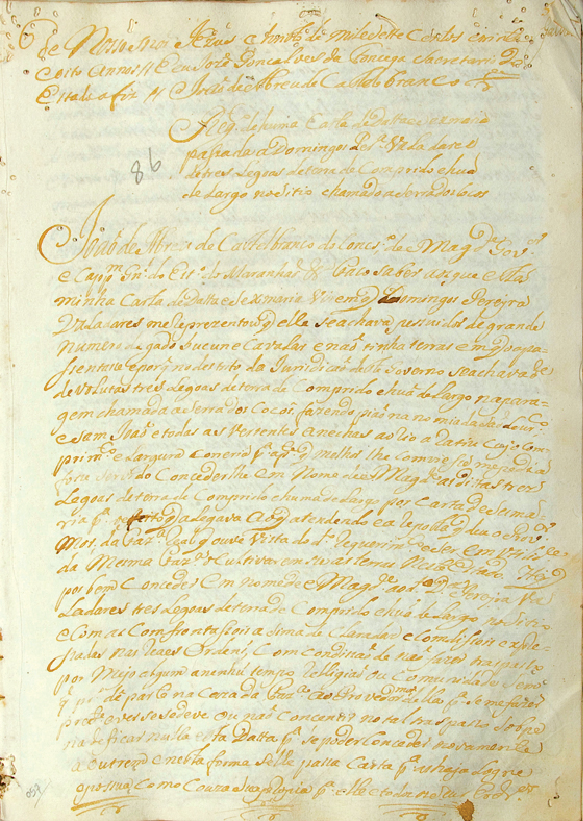
\includegraphics[width = \textwidth]
        {0167f614a7c3b3fd38127f1545dbee7c.pdf}
        \end{subfigure}
        \hspace{0.2cm}
        \qquad\tikz[baseline=-\baselineskip]\draw[ultra thick,->] (0,4) -- ++ (1,0);\qquad
        \hspace{-0.25cm}
        \begin{subfigure}[t]{0.4\textwidth}
        \centering
        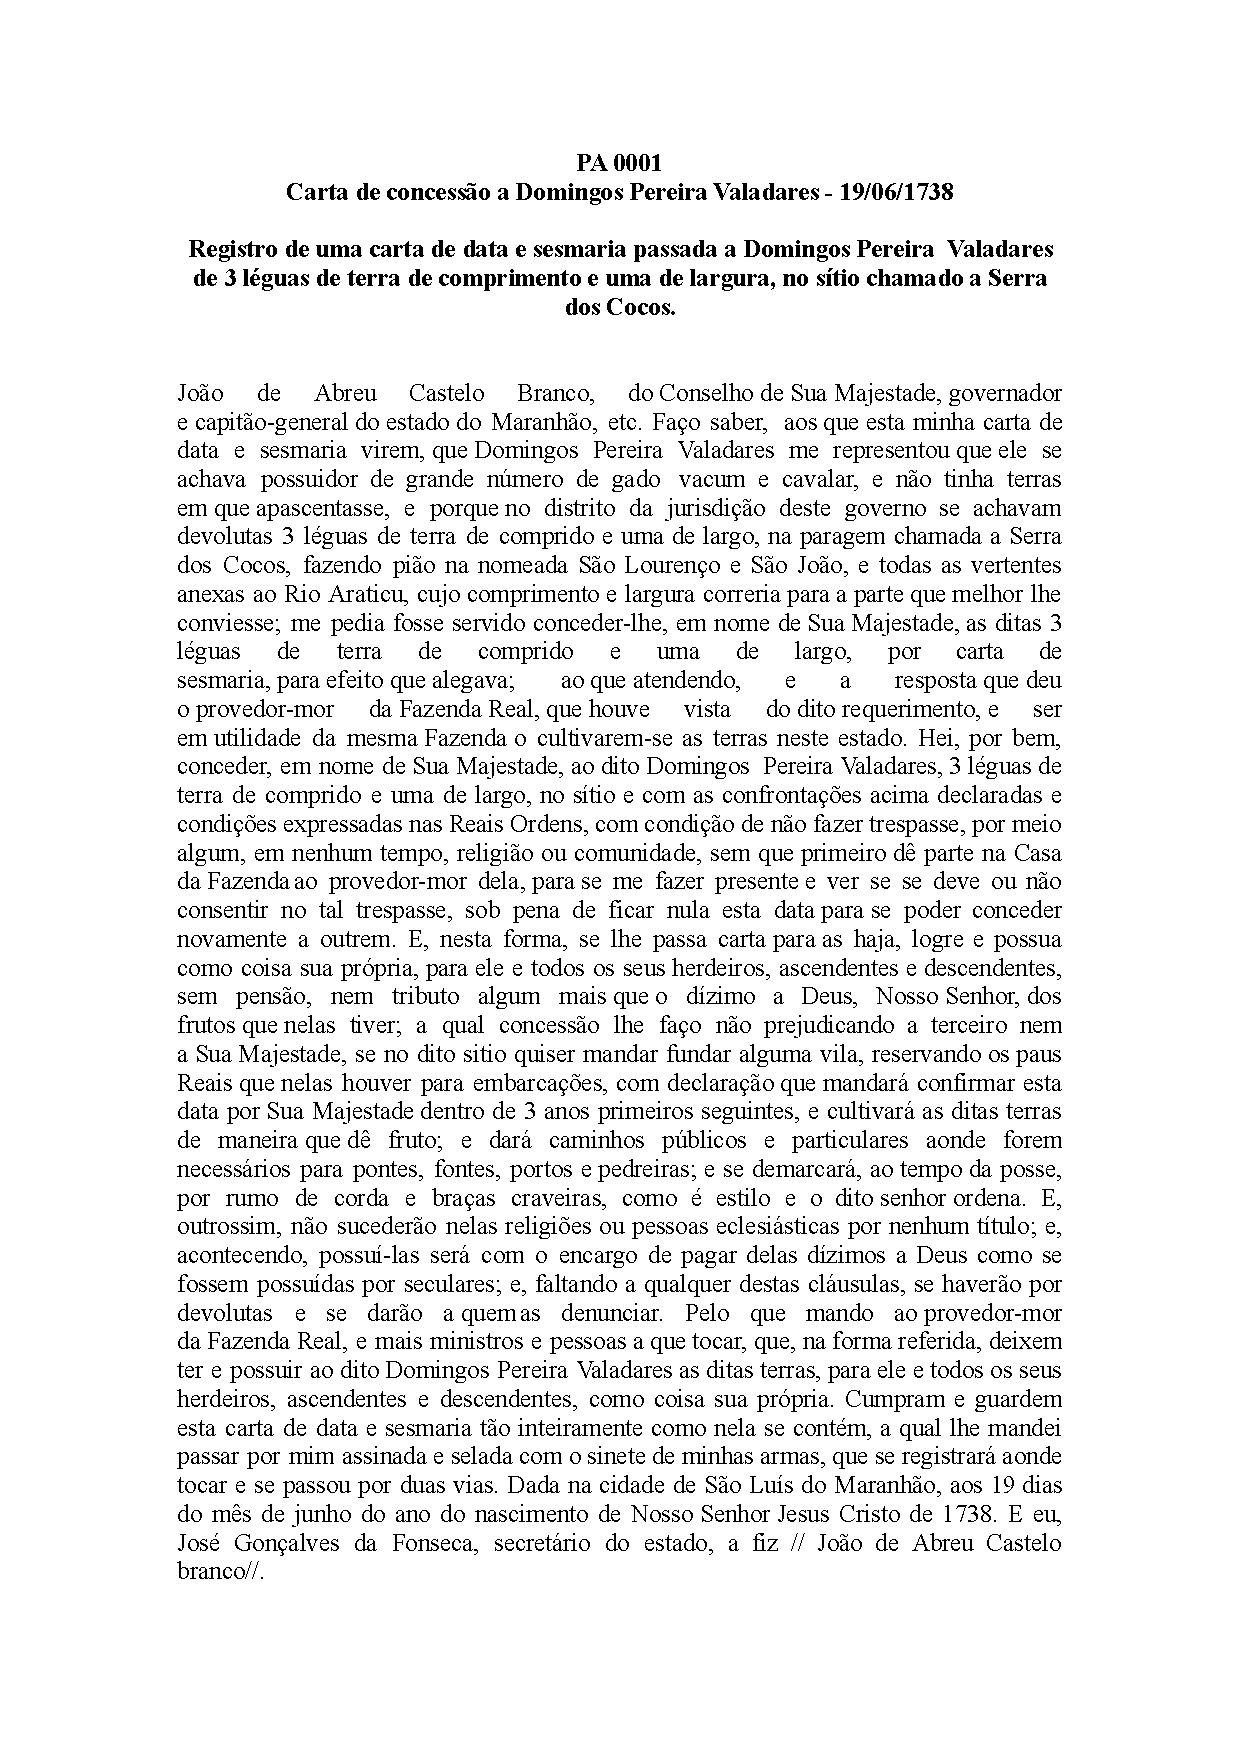
\includegraphics[page = 1, width = \textwidth]
        {ea71ea6ac7c5ec3cefa24ded60ac6438.pdf}
        \end{subfigure}
    \end{figure}
\end{frame}

% Need to create here beamer buttons so people can zoom in if they want.

% \begin{frame}{Information Extraction}
% \end{frame}

\begin{frame}{Data \hyperlink{data slide}{\beamerbutton{Back}}}
    \label{data}
    Information extracted from the letters:
    \begin{outline}
        \vspace{1mm}
        \1 Location.
        \vspace{1mm}
        \1 Year of Concession (In 1697 they were limited to 3 hectares).
        \vspace{1mm}
        \1 Type of Settler to whom it was granted.
        \vspace{1mm}
        % \1 Concessions vs. Applications
        \1 What purpose was the land requested (cattle, sugar plantation/factory, etc.).
        \vspace{1mm}
        \1 Who granted the request.
    \end{outline}
\end{frame}

\begin{frame}{Current Data Collection by State \hyperlink{work}{\beamerbutton{Back}}}
    \label{contents}
    \centering
    \includegraphics[width=0.95\textwidth,height=0.95\textheight,keepaspectratio]
    {~/OneDrive - University of Illinois - Urbana/Research/Projects/Sesmarias Brazil/Figures/Descriptive/obs_state.png}
\end{frame}


\begin{frame}{Basic Descriptive Statistics \hyperlink{work}{\beamerbutton{Back}}}{Year Dist.}
    \label{year}
    \centering
    \includegraphics[width=0.85\textwidth,height=0.85\textheight,keepaspectratio]
    {~/OneDrive - University of Illinois - Urbana/Research/Projects/Sesmarias Brazil/Figures/Descriptive/year_dist.png}
\end{frame}

\begin{frame}{Basic Descriptive Statistics (1 hec = 2.5 Football Fields) \hyperlink{work}{\beamerbutton{Back}}}{Size Dist.}
    \label{size}
    \centering
    \includegraphics[width=0.85\textwidth,height=0.85\textheight,keepaspectratio]
    {~/OneDrive - University of Illinois - Urbana/Research/Projects/Sesmarias Brazil/Figures/Descriptive/size_dist.png}
\end{frame}

\begin{frame}{Basic Descriptive Statistics (1 hec = 2.5 Football Fields) \hyperlink{work}{\beamerbutton{Back}}}{Size Dist.}
    \centering
    \includegraphics[width=0.85\textwidth,height=0.85\textheight,keepaspectratio]
    {~/OneDrive - University of Illinois - Urbana/Research/Projects/Sesmarias Brazil/Figures/Descriptive/size_dist_1697.png}
\end{frame}

\begin{frame}{Literature Review}
    \begin{outline}
        \1 Role of colonization and land tenure in present outcomes:
            \vspace{2mm}
            \2 Institutional Origins: \cite{Acemoglu2001-dz} (AER), \cite{Sokoloff2000-mb} (JEP). 
            \vspace{2mm}
            \2 Brazil: \cite{Naritomi2012-or} (JEH), 
            \cite{Musacchio2014-pq} (JEH),
            \cite{Wigton-Jones2020-ex} (JEG),
            \cite{Laudares2022-vy} (WP).
            \vspace{2mm}
            \2 India: \cites{Banerjee2005-ki} (AER).
            \vspace{2mm}
            \2 Africa: \cites{Lowes2020-pr} (WP).
    \end{outline}
\end{frame}

\end{document}